%%%%%%%%%%%%%%%%%%%%%%%%%%%%%%%%%%%%%%%%%%%%%%%%%%%%%%%%%%%%%%%%%%% 
%                                                                 %
%                            CHAPTER                              %
%                                                                 %
%%%%%%%%%%%%%%%%%%%%%%%%%%%%%%%%%%%%%%%%%%%%%%%%%%%%%%%%%%%%%%%%%%% 

\chapter{FS LS-SVM: Analysis of the Algorithm}
\section{Introduction}
In this chapter we look at the FS LS-SVM algorithm in detail.
Every block, every step along the way will get analyzed and the determination will be made if and how a parallelization is possible.
The total performance of the algorithm is discussed to decide which parts are more important.
Meaning which parts of the algorithm would benefit the most with the execution in parallel.
As described in the literature review, executing code in parallel can be divided into two mayor categories.
To simplify we name them:
\begin{itemize}
	\item GPUparallel: code/element would benefit the most of a GPU parallelization.
	\item CPUparallel: code/element eligible for CPU parallelization.
\end{itemize}
The section Linear Algebra describes how matlab can execute matrix computations in parallel, using GPUparallel or CPUparallel.
We start with an analysis of the impact of every element in the total execution time.
\section{Performance measures}
In this section a base algorithm is executed and analyzed in order to determine which elements of the algorithm takes up the most execution time.
Matlab provides a special running mode designed to do just this.
The following data set is used for the testing:
\begin{itemize}
	\item Title: Concrete Compressive Strength\cite{UCIMachi66:online}
	\item Number of attributes: 8
	\item Number of records: 1030
\end{itemize}
The number of support vectors is varied to get a better image of its influence.
The processor on my host machine is a 2,7 GHz Quad-Core Intel Core i7 with 16GB of memory available.
Under the hood Matlab actually makes use of the intelMKL library in order to already optimize the matrix computation over the available cores.
Meaning that a certain level of parallel execution is already present at this base test.
Before running the algorithm, certain values have to be chosen.
\begin{itemize}
	\item Kernel type: RBF kernel
	\item Number of support vectors: 300
	\item Number of folds: 10
	\item SV selection stop after $N/10$ unsuccessful operations.
	\item Starting $\sigma$= 0.75
\end{itemize}
Figure~\ref{fig:prato300} shows a graphical representation of the Pareto plot.
In reality both the tuning phase and support vector selection phase take about the same time. 
With a little side note that this is very dependent on the SV Selection stop criterium.
A faster stop will not only result in a faster SV selection phase but also increase the chance for a non optimal SV set, meaning that the tuning phase might take longer.
Table~\ref{tab:perf} shows the result of the same experiment with 50, 100, 300, 500 and 700 support vectors.
\begin{figure}
	\centering
	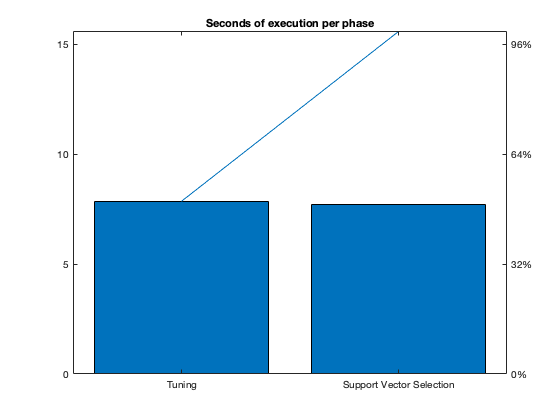
\includegraphics[width=0.8\linewidth]{pareto300.png}
	\caption{The pareto graph when 300 support vectors are used. }
	\label{fig:prato300}
\end{figure}
\begin{table}[]
	\centering
	\begin{tabular}{lll}
		Number of SV             & Selection phase {[}\%{]} & Tuning phase {[}\%{]} \\ \hline
		\multicolumn{1}{l|}{50}  & 54.1                     & 30                    \\
		\multicolumn{1}{l|}{100} & 36.6                     & 48.5                  \\
		\multicolumn{1}{l|}{300} & 48.6                     & 48.1                  \\
		\multicolumn{1}{l|}{500} & 34.1                     & 63.9                  \\
		\multicolumn{1}{l|}{700} & 16.5                     & 81.9                 
	\end{tabular}
	\caption{Values of the performance testing with variable number of SV}
	\label{tab:perf}
\end{table}
Up until 300 support vectors, the tuning phase has results in the same league as the selection phase.
The fact that Matlab uses all four CPU cores gives an advantage here, it makes the tuning phases quiet competitive.
However the performance of the selection is also determent by the fact that the lower the amount of support vector, the higher the chance for finding a better set before the stop criterium is reached, the more iteration are done.
That all being said, as you will see in the following subsection, the tuning phase has more candidates for parallel execution.
\section{Interesting Elements}
This section describes all the different elements of the FS LS-SVM algorithm.
Most of those elements are introduced in the literature review. 
Figure~\ref{fig:fslssvmDetailedOverview} gives a good overview with more details than the overview provided in figure~\ref{fig:fslssvmoverview}.
\begin{figure}
	\centering
	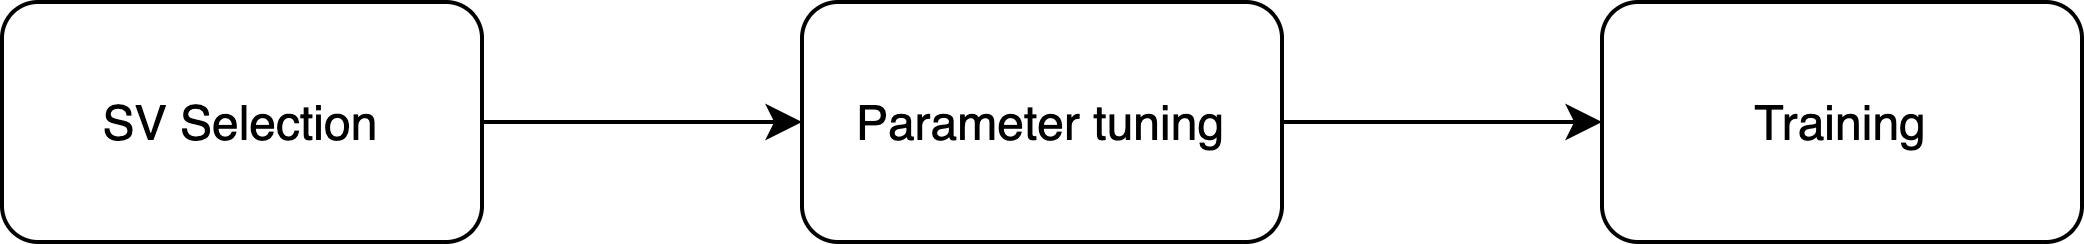
\includegraphics[width=0.8\linewidth]{fslssvm.png}
	\caption{Overview of the different phases of FS LS-SVM.}
	\label{fig:fslssvmoverview}
\end{figure}
Working from outside in, we first can distinguish three phases:
\begin{itemize}
	\item Selection: the search for the best set of support vectors.
	\item Tuning: the search for the optimal model parameters.
	\item Training: the actual model training with the correct set of support vectors and optimal parameters.
\end{itemize}
Outside the three main phases an initial block exists where the starting values and parameters are set and the use block where new data can use the generated model.
In the following subsection the different blocks of the three main phases are discussed.
\subsection{SV Selection}
As described in the literature review, the Support Vector Selection phase is in fact an iteration of the same algorithm with an acceptance phase.
The basic implementation can be found in algorithm~\ref{alg:svselection}.
\begin{algorithm}
	\fbox{\begin{minipage}{\linewidth}
			\SetKwInOut{Input}{input}\SetKwInOut{Output}{output}
			\Input{Model $model$,\\ critStart $cs$}
			\Output{Model $model$ }
			
			// initialization \\
			$Nc$ = $model.Nc$\; Nc represents the amount of support vectors wanted.
			$Xs$ = $model.X$($1$:$Nc$)\;
			$Ys$ = $model.Y$($1$:$Nc$)\;
			$critOld$ = $critStart$\;
			
			\Repeat{Until Stop conditions}{
				// First backup current candidate set \\
				$XsBackup$ =$Xs$\;
				$YsBackup$ =$Ys$\;
				// Generate new candidate set: take previous step and random swap an element \\
				$n$=random(min=1,max=size($model.X$))\;
				$nOld$=random(min=1,max=size($Xs$))\;
				$Xs$($nOld$) = $X$($n$)\;
				$Ys$($nOld$) = $Y$($n$)\;
				
				// Compute new crit value \\
				$crit$ = entropy($Xs$,$model$)\;
				
				// Acceptance condition \\
				\eIf{$crit<critold$}
				{// new candidate set is not accepted\\
					$crit$ = $critOld$\;
					$Xs$ = $XsBackup$\;
					$Ys$ = $YsBackup$\;}
				{// new candidate set is accepted\\
					$critOld$ = $crit$\;
				}	
			}
		// Final Step: assign values of Xs and Ys in model and return model
	\end{minipage}}
	\caption{Basic implementation of the support vector selection algorithm.}
	\label{alg:svselection}
\end{algorithm}
If a small alteration is made, the selection phase is a candidate for parallel execution on the CPU level.
We can state that the loop is going to execute $N$ times.
When the acceptance condition is taken out of the loop, this can be done by storing every set of indices resembling every candidate set and their corresponding criterion value, the loop can be executed in parallel.
An extra step is created because the comparison has to be done after the loop.
With a competitive sorting algorithm, the candidate set can be sorted on the criterion value with a complexity of $nlogn$, $n$ having the same value as number of iterations: $N$.
No computational high demanding matrix operations are performed in this phase, therefor it is not a suitable candidate for GPUparallel execution.
\subsection{Kernels} \label{subsec:kernels}
The function of kernel functions in LS-SVM, and more general in SVM algorithms, is discussed in the literature review.
However in FS LS-SVM the kernel function is computed for the completed data set based only on a selection.
The exact selection that is made by the support vector selection algorithm and handed as an input in this section.
The following assumptions are made:
\begin{itemize}
	\item The complete set of data point consists of $n$ items.
	\item The subset of data points (the selected support vectors) consists of $m$ items.
	\item The specific kernel function that is used in this thesis is called \textit{RBF kernel}, more information and the equation can be found in section~\ref{subsec:kerneltrick}.
	\item The kernel matrix that is constructed will be referred to as $\Omega$.
	\item The features matrix will be referred to as $\Phi$.
\end{itemize}
In the normal LS-SVM approach, the kernel matrix $\Omega$ constructed would be of a dimension $n$x$n$, because of the fact that all $n$ data points are considered support vectors.
With FS LS-SVM, the dimension of $\Omega$ is reduced to $n$x$m$.
This reduces the memory complexity from $\mathcal{O}(n^2)$ to $\mathcal{O}(nm)$, which is significant because $m<<<n$.
\par 
In the FS LS-SVM algorithm the extended feature matrix $\hat{\Phi_e}$ is used.
This matrix represents the bridge in the feature space between the complete data set and the selected support vectors.
To compute this $\hat{\Phi_e}$, a couple of things are required: 
\begin{itemize}
	\item The kernel matrix of the support vectors: $\Omega$.
	\item The kernel matrix between the complete data set and the support vectors $\Omega_N$.
	\item The eigendecomposition of kernel matrix $\Omega$.
\end{itemize}
The Nystr\"om method combines these elements into the features matrix $\hat{\Phi_e}$, as shown in equation~\ref{eq:nystrom}.
\begin{equation}
	\hat{\Phi_e}= repmat(\frac{1}{\sqrt{eigvals(\Omega)}},n).*\Omega_N eigvecs(\Omega)
	\label{eq:nystrom}
\end{equation}
To compute this $\hat{\Phi_e}$, a bunch of matrix operations are needed.
All these operations have their own time and memory complexity that are still strongly dependent on input size $n$, making it a very heavy computational part of the algorithm.
The complexities of each computation is shown in table~\ref{tab:featurescomplexity}.
Figure~\ref{fig:nystrom} shows the feature extraction steps following the Nystr\"om method.
\begin{figure}
	\centering
	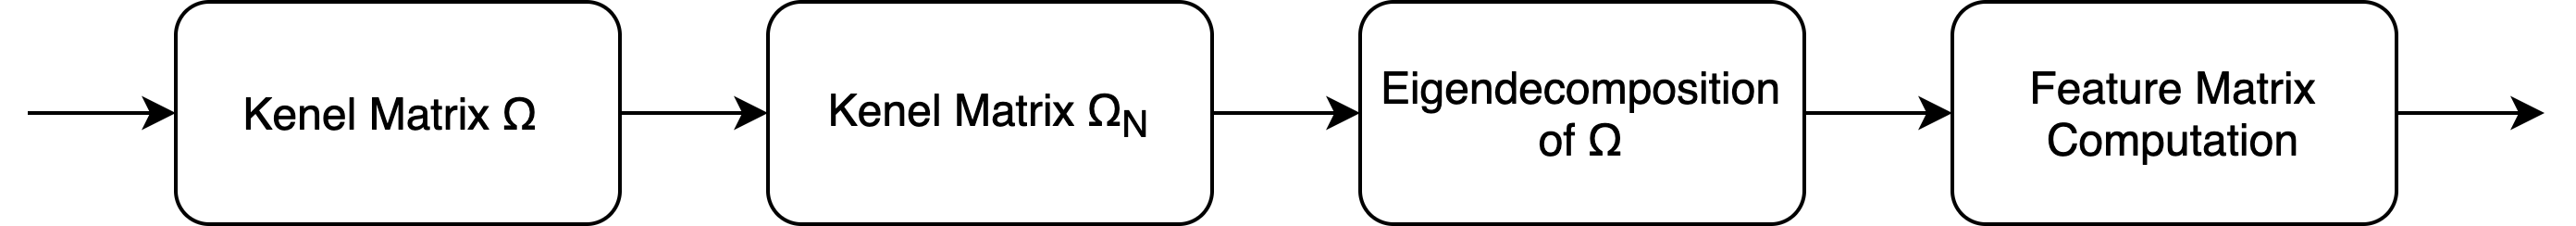
\includegraphics[width=\linewidth]{fastvfoldcrossvalidation.png}
	\caption{Graphical representation of the sequential steps taken in the Nystr\"om method.}
	\label{fig:nystrom}
\end{figure}
\begin{table}[]
	\centering
	\begin{tabular}{lll}
		& Computation Complexity & Memory Complexity  \\ \hline
		\multicolumn{1}{l|}{Kernel Matrix $\Omega$}         & $\mathcal{O}(nm)$      & $\mathcal{O}(nm)$  \\
		\multicolumn{1}{l|}{Kernel Matrix $\Omega_N$}       & $\mathcal{O}(nm)$      & $\mathcal{O}(nm)$  \\
		\multicolumn{1}{l|}{Eigendecomposition of $\Omega$} & $\mathcal{O}(m^3)$     & $\mathcal{O}(m^2)$ \\
		\multicolumn{1}{l|}{Feature Matrix $\hat{\Phi_e}$}  & $\mathcal{O}(nm^2)$    & $\mathcal{O}(nm)$ 
	\end{tabular}
	\caption{Time and memory complexity of the matrix computations used to calculate the feature matrix.}
	\label{tab:featurescomplexity}
\end{table}
Each of those computation is a good candidate for GPUparallel execution.
\subsection{Coupled Simulating Annealing}
CSA is described in detail in the literature review. 
Multiple variants were also introduced, mostly making a difference in the calculation of cost functions.
Often this optimization algorithm is described as $n$\footnote{In this section $n$ does not stand for the number of input data points but it represents the number of coupled values in CSA.} parallel channels of the base SA algorithm coupled together in the cost function.
In my opinion this description can give a good context but is not entirely correct.
In reality it can better be described as a single SA algorithm but instead of taking only one candidate value at a time, it takes $n$.
This does make a big difference for me.
The first formulation suggest that multiple parallel paths can be created that in certain moments have to communicate which each other.
What strongly leans to CPUparallel execution with shared memory.
This is in fact not the case, a single thread has to execute the learning loop, only the calculation of cost values at each evaluation is a candidate for parallel execution.
To make this more clear figure~\ref{fig:parallelcsa} shows a visual representation of the two concepts.
\begin{figure}
	\centering
	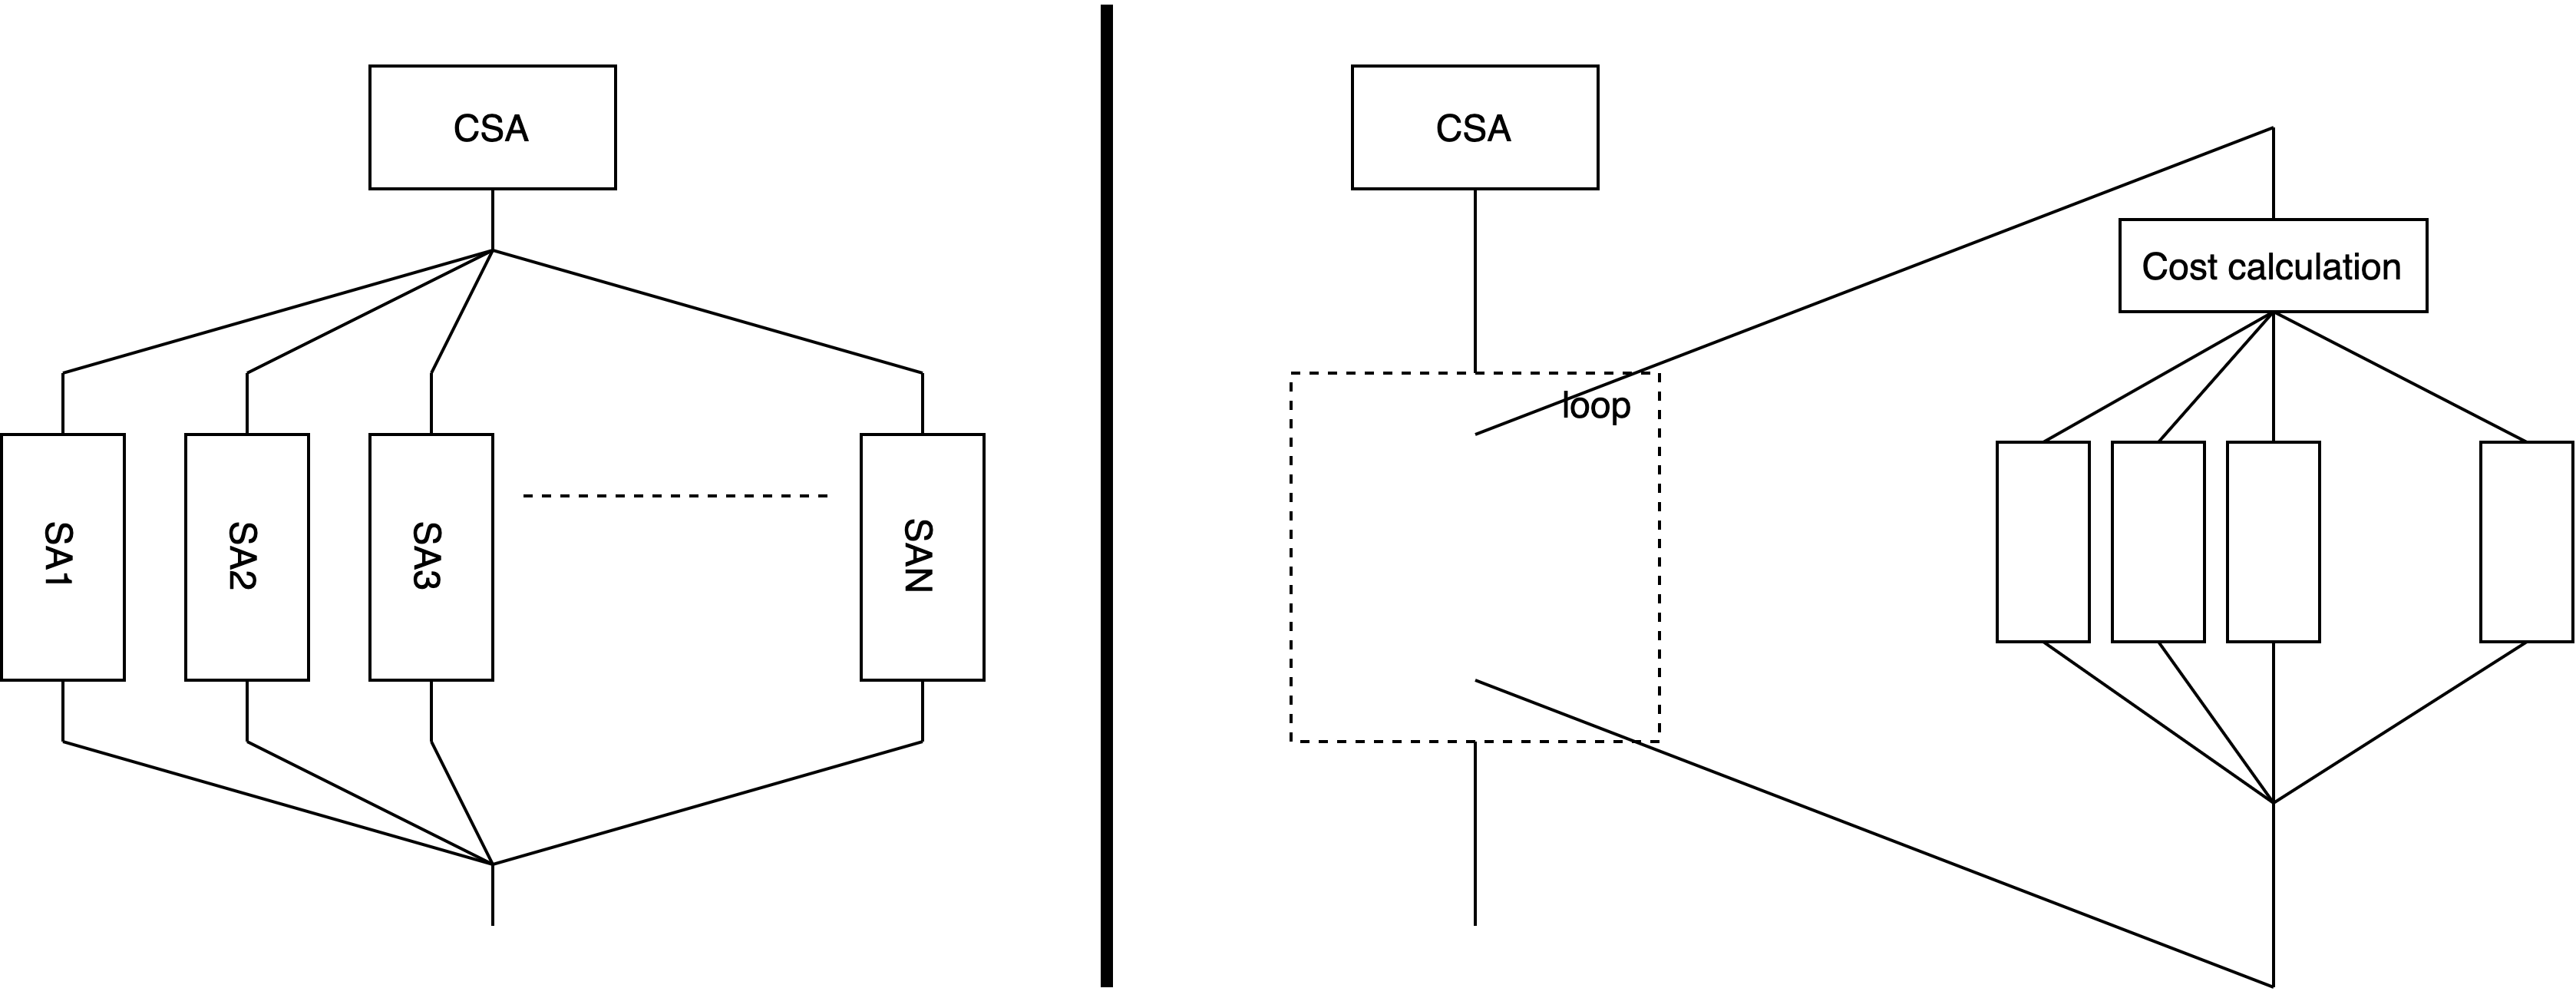
\includegraphics[width=\linewidth]{parallelcsa.png}
	\caption{Left a visualization of csa that is not correct; Right a visualization of parallel csa that comes closer to reality.}
	\label{fig:parallelcsa}
\end{figure}
\par 
If these concepts are clear, we can understand that the CSA algorithm itself does not have parallel execution potential.
However the cost calculation function does have that potential.
In FS LS-SVM and with extension the optimized version \cite{Optimized2010:article}, the cost of a possible solution found by CSA is calculated by the \textit{fast v-fold crossvalidation} algorithm.
Any parallel execution potential of CSA is depended on this function. 
\subsection{Simplex}
The simplex algorithm is used in FS LS-SVM to narrow down the suggestion CSA made for parameter values.
With the objective to find the true optimal values.
When we look at parallelization potential, we see a similar story as with CSA.
The core of the search heuristic consists of a loop that is depended on the result of the previous iteration.
Making it unsuitable for CPUparallel as wel as GPUparallel execution.
However the simplex function also makes use of a cost function and in this case the same function as CSA uses: \textit{fast v-fold crossvalidation}.
This results in the fact that both CSA and simplex export the interesting elements for parallel execution to the same cost function.
\subsection{Crossvalidation}
As described earlier both CSA and simplex heavily rely on a crossvalidation function to calculate the cost of a possible solution.
In the optimized FS LS-SVM the specific crossvalidation function is called \textit{fast v-fold crossvalidation}.
\textit{Fast v-fold crossvalidation} is earlier described in the literature review, this section focuses on the mathematical computations done as well as possible parallel streams.
\paragraph{J Couples}
When we start with a look from the outside, a first thing we notice is that both the CSA and simplex search heuristic send (multiple) couples of values to the crossvalidation algorithm to get a representative performance score.
Meaning that a matrix with dimension $j$x$2$ is sent with input values, the crossvalidation has to run $j$ times, compute an individual score for each entry and at the end combine those scores in to one final representative score for the input set.
This is a perfect case for CPUparallel execution: $j$ different parallel execution paths, independent from each other. 
Of course before exiting the crossvalidation function, the parallel region has to end and a single thread has to execute the combination of the $j$ different scores.
\paragraph{V Folds} 
Diving into a single crossvalidation, we can actually see the same thing happening.
The algorithm consists of a loop that will be executed $v$ times, every time with a different training and validation set.
However the computations done in this loop are not dependent on each other and therefore parallel execution is perfectly possible.
In other words this is also a candidate for CPUparallel code execution.
One iteration of this loop is called a fold, hence the name \textit{fast v-fold crossvalidation}.
\par 
Before the $v$ parallel folds can be started, the feature matrix $\hat{\Phi_e}$, $A$ and $C$ need to be calculated.
This is because every fold takes the complete feature matrix as an input argument, together with the from $\hat{\Phi_e}$ derived matrices $A$ and $C$.
As described in section~\ref{subsec:kernels}, and shown in figure~\ref{fig:nystrom}, this feature extraction consists of a certain amount of sequential steps.
Each step consisting of demanding matrix operations, the complexity is listed in table~\ref{tab:featurescomplexity}.
Every step of this Nystr\"om method is a candidate for GPUparallel code execution.
As shown in figure~\ref{fig:prefold}, after the Nystr\"om method is done, two more computations need to be done before the $v$ folds can start.
These computations, matrix A and C computation, are both candidates for parallel execution and can be calculated at the same time if multiple GPUs are available (or enough GPU cores).
The equations used how to calculate the matrices A and C are shown in section~\ref{subsec:fastvfoldcv}.
Time and memory complexity of both computations is shown in table~\ref{tab:prefold}.
\begin{table}[]
	\centering
	\begin{tabular}{lll}
		& Time Complexity     & Memory Complexity  \\ \hline
		\multicolumn{1}{l|}{Matrix A} & $\mathcal{O}(nm^2)$ & $\mathcal{O}(m^2)$ \\
		\multicolumn{1}{l|}{Vector c} & $\mathcal{O}(nm)$   & $\mathcal{O}(m)$  
	\end{tabular}
	\caption{Time and memory complexity of the prefold calculations}
	\label{tab:prefold}
\end{table}
\begin{figure}
	\centering
	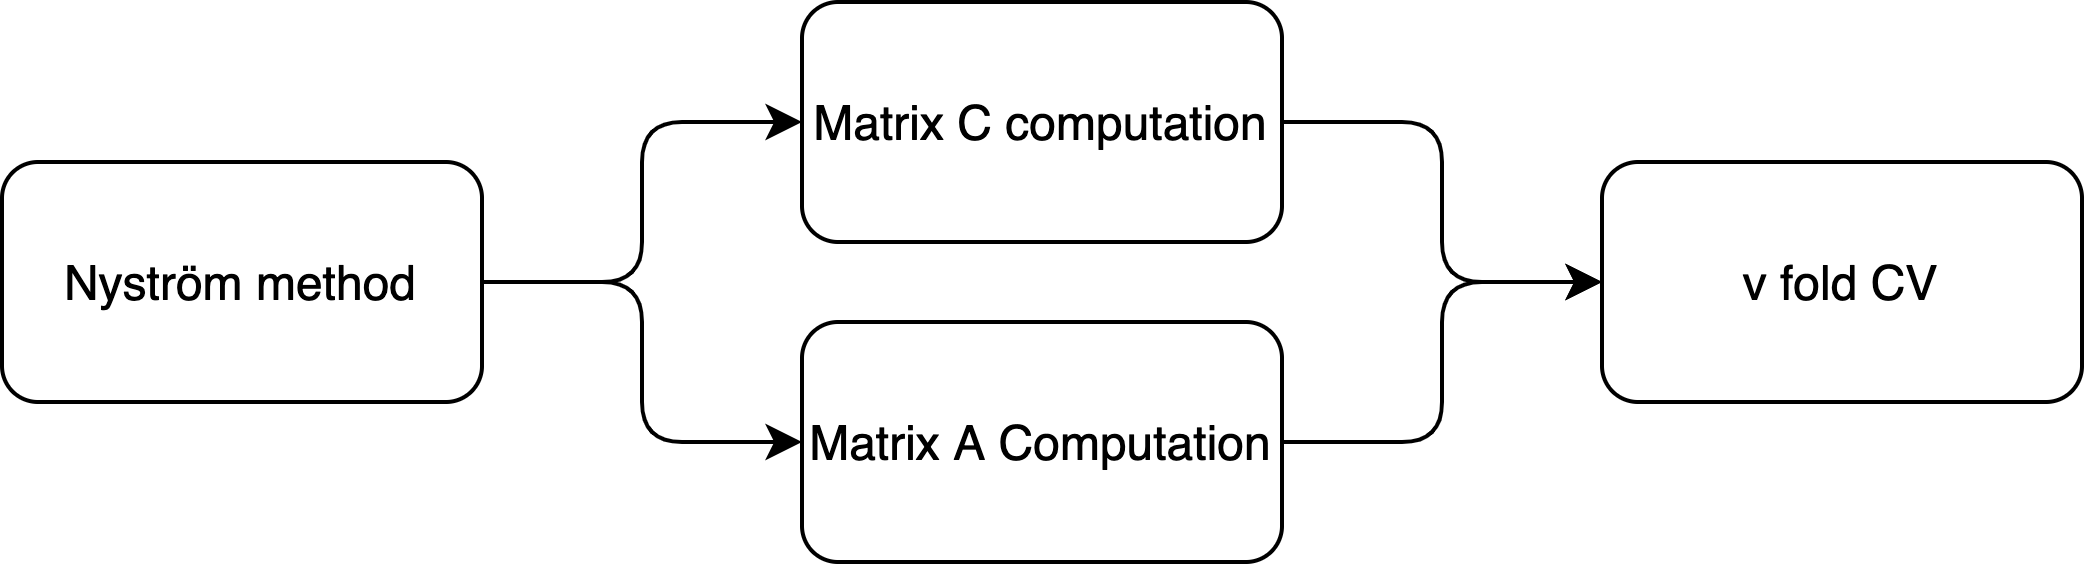
\includegraphics[width=\linewidth]{fastvfoldcrossvalidationAC.png}
	\caption{Graphic representation of the computation steps done before starting the folds.}
	\label{fig:prefold}
\end{figure}
\paragraph{Single Fold}
Every single fold gets the same input arguments: 
\begin{itemize}
	\item Feature matrix $\hat{\Phi_e}$
	\item Trainig data set
	\item fold number $v$
	\item Complete matrix A
	\item Complete vector c
\end{itemize}
Figure~\ref{fig:singleFold} shows the steps taken in a single fold.
Matrix $A_v$ computation, Vector $c_v$ computation and the Linear Equation Solving are suitable candidates for GPUparalle execution.
They are in fact just matrix operations.
Equation~\ref{eq:linearsystemfold} shows the linear Equation Solving, taking as an input both $Av$ and $Cv$.
Equation~\ref{eq:Avfold} shows how to compute $A_v$.
Equation~\ref{eq:cvfold} shows how to compute $c_v$.

\begin{figure}
	\centering
	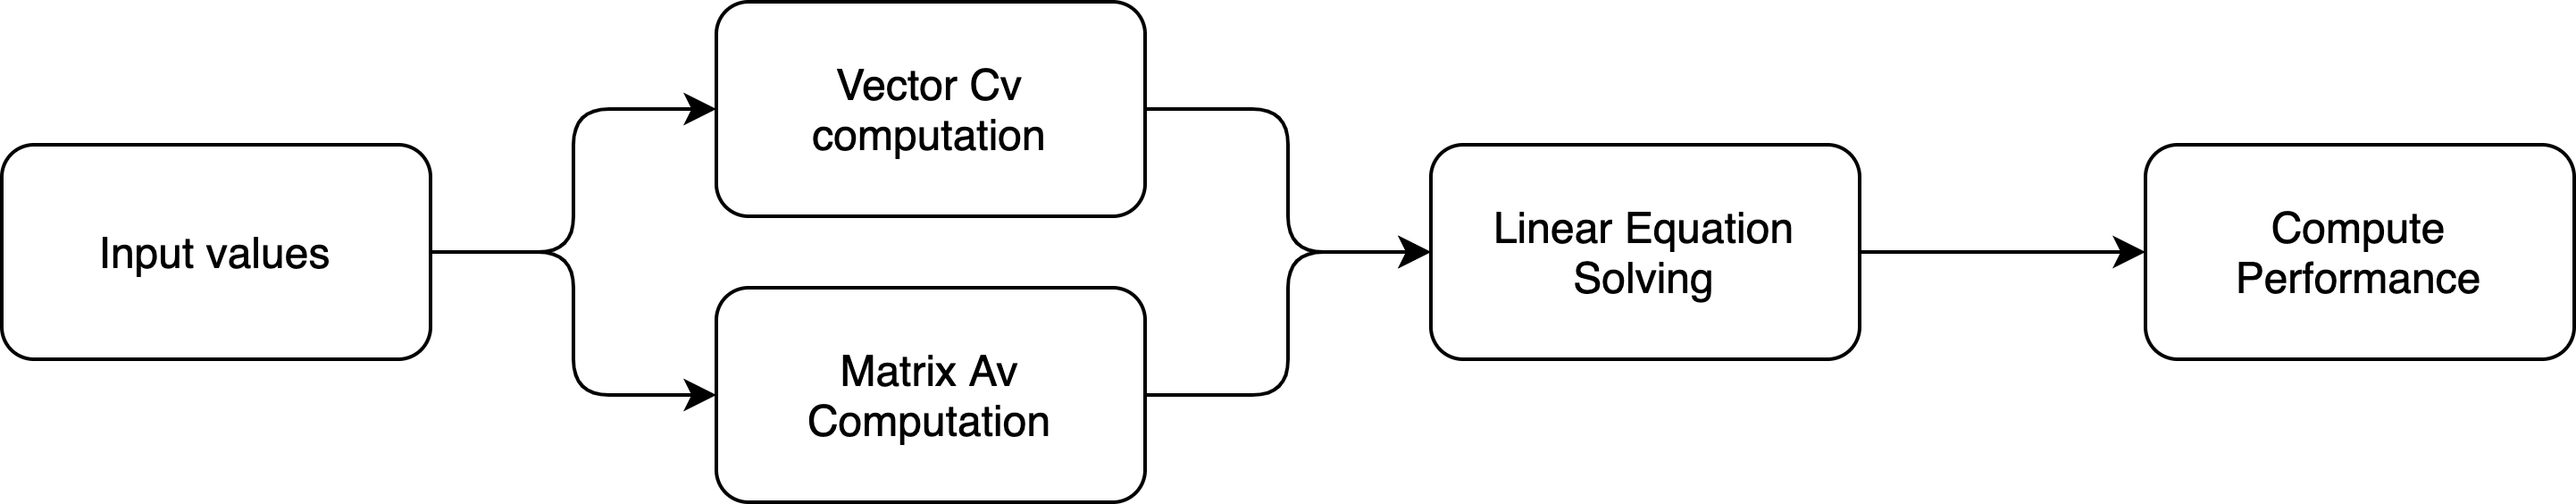
\includegraphics[width=\linewidth]{fastvfoldcrossvalidationSingleFold.png}
	\caption{Graphical representation of the steps in a single fold.}
	\label{fig:singleFold}
\end{figure}
\begin{equation}
	\binom{\hat{w}}{\hat{b}} = A_v^{-1}c_v
	\label{eq:linearsystemfold}
\end{equation}
\begin{equation}
	A_v = A - \left(\frac{\hat{\Phi}_{val}^T}{1_{val}^T}\right)  \left(\hat{\Phi}_{val} 1_{val}\right)
	\label{eq:Avfold}
\end{equation}
\begin{equation}
	c_v = c - \left(\frac{\hat{\Phi}_{val}^T}{1_{val}^T}\right)Y_{val}
	\label{eq:cvfold}
\end{equation}
For the first time a parallel execution difficulty occurs.
When executing both $J$ couples and $v$ folds in CPU parallel, a nested parallel execution is created.
This is a difficulty because a distribution has to be chosen, the available parallel streams have to be divided between the needed paths.
When a equal distribution is chosen and for example four parallel paths can be created, the situation is described in figure~\ref{fig:nestedparallel}.
\par
The second parallel execution difficulty that occurs is the possible simultanious computation of $A$ - $c$ and $A_v$ - $c_v$.
This is theoretically possible but not easy to achieve in Matlab, where in the end there is limited control over what ends up where and is executed how on the GPU.
\begin{figure}
	\centering
	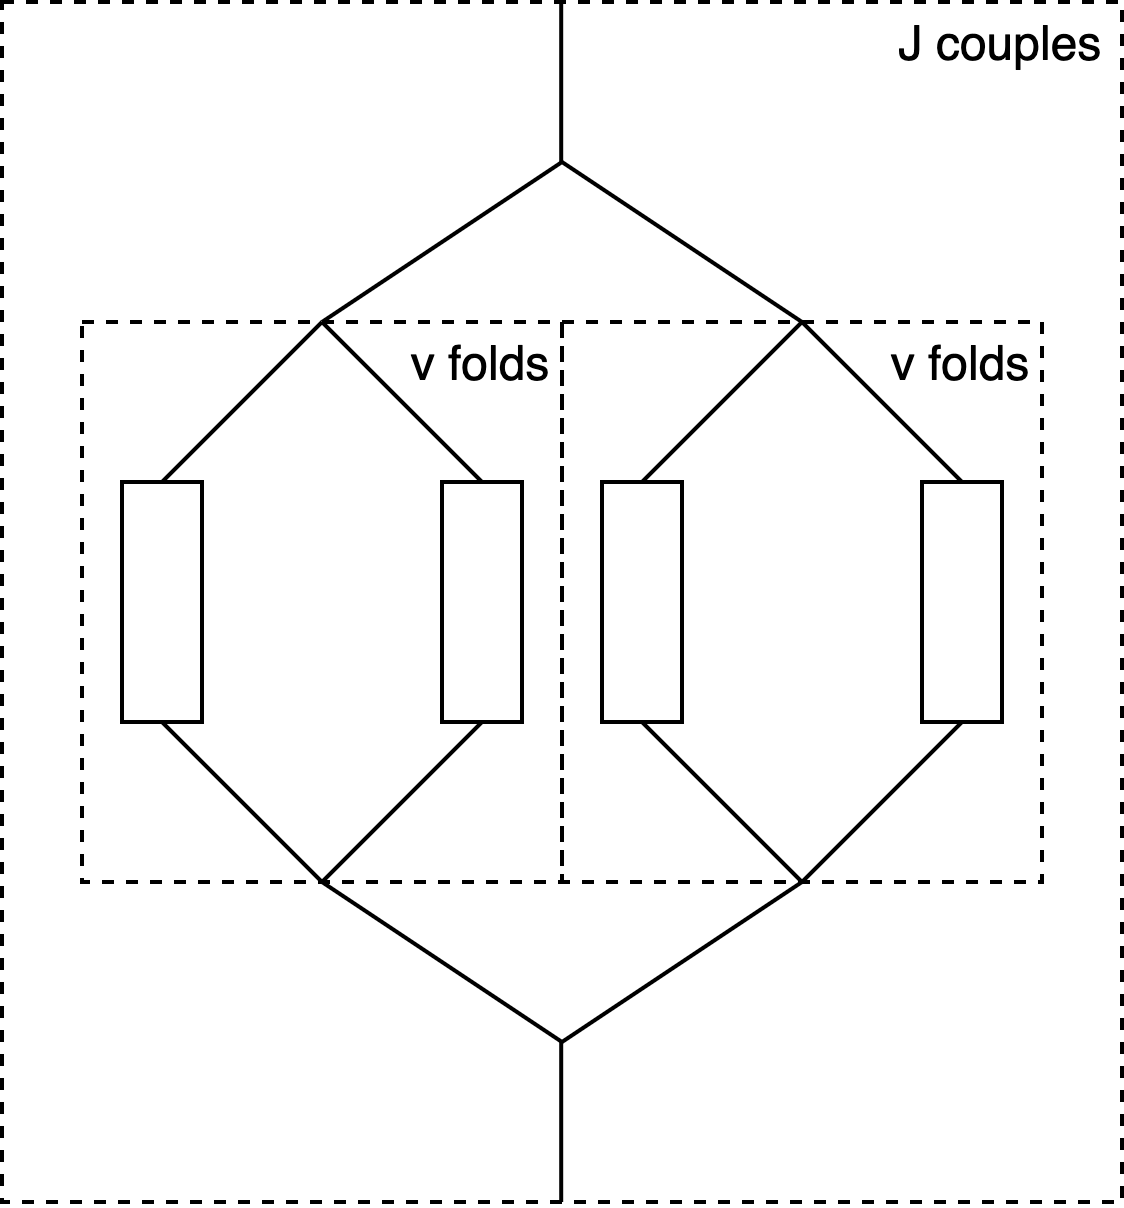
\includegraphics[width=0.8\linewidth]{nestedparallel.png}
	\caption{Graphical representation of the nested parallel region.}
	\label{fig:nestedparallel}
\end{figure}
\section{Conclusion}
Looking at the complete picture, multiple elements qualify for parallel execution.
Both CPUparallel and GPUparallel execution.
Table~\ref{tab:parcandidates} shows a complete lists of all the elements.
An extra layer to add is that this analysis covered the core of the algorithm.
Extra elements might appear when choosing a certain use case, meaning that function estimation, classification and multi-classification each have their specific logic at some points.
Especially when looking at multi-classification, depending on the chosen coding, a certain amount of models have to be created. 
Each of these models can be calculated in parallel of each other as they actually do not depend on data from each other.
Another side note is the competitiveness of models.
In certain cases to enhance the competitiveness of a solution, multiple models are created for the same case and the one with the highest performance score (or lowest error score) is chosen as a final solution.
If that is applied, it can be done perfectly in parallel streams.
When speaking about multi-classification and competitiveness we are in both cases talking about CPUparallel code execution possibilities.
\par 
Returning to table~\ref{tab:parcandidates}, as earlier described there are two different categories: CPUparallel and GPUparallel.
Each candidate is given a status for those two categories.
The possibilities for a status are: possible, possible yet not ideal and not possible.
Those three statuses are possible because every matrix operation can be executed in parallel on a CPU, only this is not ideal.
The performance gain by executing matrix operation in parallel on a GPU is much larger, hence the possible yet not ideal CPUparallel status for every candidate that has a GPUparallel possible status.
\par
Two parallel execution difficulties made their introduction in certain elements: nested parallel and simultaneous GPU execution. 
\begin{table}[]
	\centering
	\begin{tabular}{lll}
		& CPUparallel            & GPUparallel  \\ \hline
		\multicolumn{1}{l|}{SV selection}                        & possible               & not possible \\
		\multicolumn{1}{l|}{$J$ couples}                         & possible               & not possible \\
		\multicolumn{1}{l|}{Kernel Matrix $\Omega$}              & possible yet not ideal & possible     \\
		\multicolumn{1}{l|}{Kernel Matrix $\Omega_N$}            & possible yet not ideal & possible     \\
		\multicolumn{1}{l|}{Eigendecomposition of $\Omega$}      & possible yet not ideal & possible     \\
		\multicolumn{1}{l|}{Features Computation $\hat{\Phi}_e$} & possible yet not ideal & possible     \\
		\multicolumn{1}{l|}{Matrix A}                            & possible yet not ideal & possible     \\
		\multicolumn{1}{l|}{Vector c}                            & possible yet not ideal & possible     \\
		\multicolumn{1}{l|}{$V$ folds}                           & possible               & not possible \\
		\multicolumn{1}{l|}{Matrix $A_v$}                        & possible yet not ideal & possible     \\
		\multicolumn{1}{l|}{Vector $c_v$}                        & possible yet not ideal & possible     \\
		\multicolumn{1}{l|}{Linear System Solving}               & possible yet not ideal & possible    
	\end{tabular}
	\caption{List of elements that can be executed in parallel.}
	\label{tab:parcandidates}
\end{table}